\documentclass[dvipsnames,png,border=10pt,tikz]{article}
\usepackage{tikz}
\usetikzlibrary{shapes.geometric} % required for the ellipse shape
%\usetikzlibrary{arrows, backgrounds, calc, hobby, positioning}



\usepackage{pgf}
\usepackage{tikz}
\usetikzlibrary{calc,arrows,decorations.pathmorphing,backgrounds,positioning,fit,petri,automata,shadings,shadows}


\tikzset{vertex style/.style={
    draw=#1,
    thick,
    fill=#1!70,
    text=white,
    ellipse,
    minimum width=2cm,
    minimum height=0.75cm,
    font=\small,
    outer sep=3pt,
  },
  text style/.style={
    sloped,
    text=black,
    font=\footnotesize,
    above
  }
}

\tikzstyle{literals}=[draw,circle,violet,bottom color=\lav,
                  top color= white, text=violet,minimum width=10pt]
\tikzstyle{superpeers}=[draw,circle,burntorange, left color=\oran,
                       text=violet,minimum width=20pt]
\tikzstyle{legendsp}=[rectangle, draw, burntorange, rounded corners,
                     thin,bottom color=\oran, top color=white,
                     text=burntorange, minimum width=2.5cm]
\tikzstyle{legendp}=[rectangle, draw, violet, rounded corners, thin,
                     bottom color=\lav, top color= white,
                     text= violet, minimum width= 2.5cm]
\tikzstyle{legend_general}=[rectangle, rounded corners, thin,
                           burntorange, fill= white, draw, text=violet,
                           minimum width=2.5cm, minimum height=0.8cm]
                           
                           

\begin{document}
% \begin{tikzpicture}[node distance=2.75cm,>=stealth']
% \node[vertex style=Turquoise] (Rk) {rdfindex-wb:TheWorldBankNaiveIndex};
% 
% \node[vertex style=BurntOrange, above of=Rk,xshift=2em] (BD) {"The Weight Longest Life Country"@en}
%  edge [<-,cyan!60!blue] node[text style]{rdfs:label} (Rk);
% 
% \node[vertex style=BurntOrange, right=1.5cm of Rk,yshift=4ex] (AP) {rdfindex:Quantitative}
%  edge [<-,cyan!60!blue] node[text style]{rdfindex:type} (Rk); 
% 
% \node[vertex style=red, below right of=Rk,xshift=3em] (JA) {John Avnet}
%  edge [<-,cyan!60!blue] node[text style]{rdfindex:aggregates} (Rk); 
% 
% 
% \end{tikzpicture}


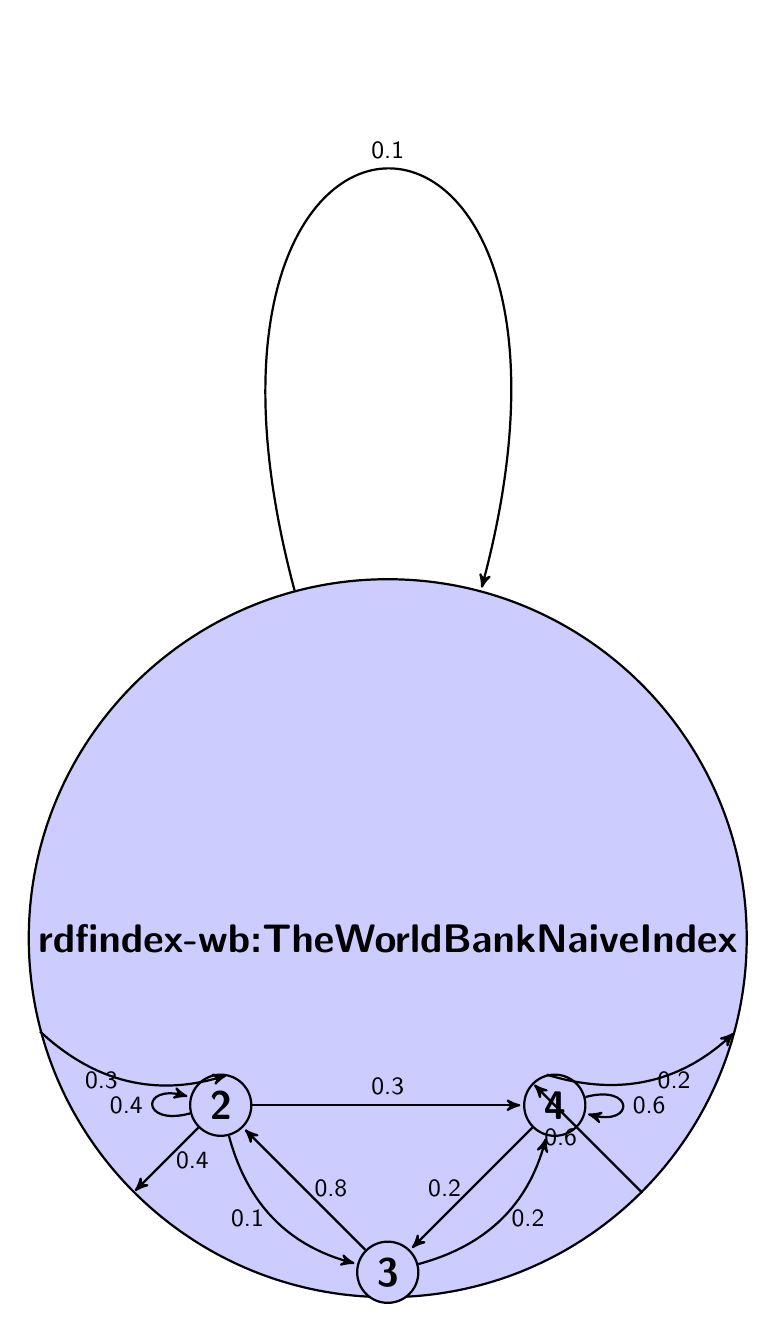
\begin{tikzpicture}[->,>=stealth',shorten >=1pt,auto,node distance=3cm,
  thick,main node/.style={circle,fill=blue!20,draw,font=\sffamily\Large\bfseries}]

  \node[main node] (1) {rdfindex-wb:TheWorldBankNaiveIndex};
  \node[main node] (2) [below left of=1] {2};
  \node[main node] (3) [below right of=2] {3};
  \node[main node] (4) [below right of=1] {4};

  \path[every node/.style={font=\sffamily\small}]
    (1) edge node [left] {0.6} (4)
        edge [bend right] node[left] {0.3} (2)
        edge [loop above] node {0.1} (1)
    (2) edge node [right] {0.4} (1)
        edge node {0.3} (4)
        edge [loop left] node {0.4} (2)
        edge [bend right] node[left] {0.1} (3)
    (3) edge node [right] {0.8} (2)
        edge [bend right] node[right] {0.2} (4)
    (4) edge node [left] {0.2} (3)
        edge [loop right] node {0.6} (4)
        edge [bend right] node[right] {0.2} (1);
\end{tikzpicture}


% rdfindex-wb:TheWorldBankNaiveIndex 
%   a rdfindex:Index;
%   rdfs:label "The Weight Longest Life Country"@en;
%   rdfindex:type rdfindex:Quantitative;
%   rdfindex:aggregates [ 		
%     rdfindex:aggregation-operator rdfindex:OWA;
%     rdfindex:part-of [
%       rdfindex:dataset rdfindex-wb:AidEffectiveness; 
%       rdfindex:weight 0.4];
%     rdfindex:part-of [rdfindex:dataset rdfindex-wb:Health; 
%       rdfindex:weight 0.6];
%   ];
%   #More metadata properties...
%   qb:structure 	rdfindex-wb:TheWorldBankNaiveIndexDSD ; .
%   
% rdfindex-wb:TheWorldBankNaiveIndexDSD 
%   a qb:DataStructureDefinition;  
%   qb:component    
%   [qb:dimension rdfindex-wbont:ref-area],
%   [qb:dimension rdfindex-wbont:ref-year],
%   [qb:measure   rdfindex:value],
%   [qb:attribute sdmx-attribute:unitMeasure];
%   #More metadata properties...
  


\end{document}